\documentclass[10pt,letterpaper]{article}

\usepackage{cogsci}
\usepackage{pslatex}
\usepackage[nodoi]{apacite}
\usepackage{graphicx}
\usepackage[raggedright]{sidecap}

%\graphicspath{plots/}
%\usepackage{float}
% \usepackage{subcaption}
% \usepackage{lipsum}
% \usepackage{hyperref}
% \usepackage[section]{placeins}
% \usepackage[font=footnotesize,skip=0pt]{caption}
% \usepackage{stfloats}

% \setcounter{topnumber}{2}
% \setcounter{bottomnumber}{2}
% \setcounter{totalnumber}{4}
% \renewcommand{\topfraction}{0.85}
% \renewcommand{\bottomfraction}{0.85}
% \renewcommand{\textfraction}{0.15}
% \renewcommand{\floatpagefraction}{0.7}

\title{Developmental Changes in the Relationship Between Grammar and the Lexicon}
% \title{Developmental Change in the Relationship Between Lexical and Grammatical Acquisition}
 
\author{{\large \bf Mika Braginsky} \\
  \texttt{mikabr@stanford.edu} \\
  Department of Psychology \\
  Stanford University
  \And {\large \bf Daniel Yurovsky} \\
  \texttt{yurovsky@stanford.edu} \\
  Department of Psychology \\
  Stanford University
    \And {\large \bf Virginia Marchman} \\
    \texttt{marchman@stanford.edu} \\
  Department of Psychology \\
  Stanford University
    \And {\large \bf Michael C. Frank}\\
    \texttt{mcfrank@stanford.edu} \\
  Department of Psychology \\
  Stanford University}


\begin{document}

\maketitle

\begin{abstract}


\textbf{Keywords:} 
Language acquisition; word learning; syntax; development
\end{abstract}

\section{Introduction}

Does abstract structure in language emerge from the interaction of individual words, or are syntactic structures represented separately? On lexicalist theories of grammatical development, syntactic structure emerges from graded generalizations on the basis of lexical items and there may be little or no representation of syntactic rules or regularities per se, at least early in development \cite{tomasello2001,tomasello2003}. Even if syntactic structures are eventually represented, these representations should be directly related to their support in more concrete lexical structure \cite{bannard2009,borensztajn2008}. In contrast, on more nativist theories like principles and parameters \cite{chomsky1981, baker2005}, grammar is predicted to emerge independently from lexical knowledge and on its own (largely maturational) timetable. On these theories, older children should have more syntactic competence, largely independent from the amount of language input they receive and hence from the size of their vocabulary.

By providing estimates of the relationship between grammar, lexicon, and age,  developmental data can help resolve this conflict. Analyses of data from the MacArthur-Bates Communicative Development Inventory (CDI; a widely-used parent report language measure) show a systematic relationship between the number of words that a child knows and their grammatical knowledge, as estimated via a set of checklist items relating to the complexity of sentence production \cite{bates1997,caselli1999}. While each of these measures---vocabulary and complexity checklist responses---both have been found to be reliable and valid measures of early child language \cite{fenson1994,fenson2007}.  This consistent non-linear relationship means that the size of the lexicon accurately predicts a measure of grammar, providing initial support for lexicalist theories of acquisition.

On the other hand, this initial work did not have the statistical power to test the hypothesis that there was additional age-related variance in syntactic development that was unexplained by vocabulary. Given that age-based changes would suggest the presence of developmental processes that regulate grammatical acquisition above and beyond lexical acquisition, such changes would provide an important signal about other contributors to syntactic acquisition. We take up this hypothesis in our current work. 

We probe the lexicon-grammar relationship further by delineating grammatical development into more targeted measures that 1) capture distinctions between morphological and syntactic knowledge; and 2) characterize the composition of the lexicon by grammatical function. For each of these, we examine the relationship between the measure and the size of the lexicon, and determine how age affects the relationship. A measure's relationship not changing with age indicates that vocabulary size predicts it thoroughly, while age-related change is indicative of the presence of some developmental shift not captured by vocabulary size.

Our measures of both lexical and grammatical development are derived from the CDI. The CDI is an inexpensive data-gathering method and has the advantages that large pre-existing samples already exist for a number of languages. We use data here from 19,822 administrations of CDI Toddler forms, taken from Wordbank, a new website for aggregating CDI data into a consistent format across forms and languages. We use data from adaptations of the CDI into four languages: English, Spanish, Norwegian, and Danish to establish cross-linguistic generalizability to our findings.

Each language's adaptation of the CDI includes a vocabulary checklist, a word form section consisting of morphological inflections, and a complexity section consisting of pairs of syntactically simple/complex sentences. Vocabulary size as measured by the CDI correlates with both laboratory measurements and naturalistic observation (see \cite{fenson2007} for a review) and score on the complexity section correlates with MLU and other measurements of grammatical development.

We begin by describing the Wordbank database, the CDI measures we make use of, and our general analytic approach. We then describe two sets of analyses of the relationship of age to the links between grammar and the lexicon. The first examines the relationship between vocabulary (measured by the production checklist items of the CDI) and morphological and grammatical complexity. The second takes advantage of the a theoretical prediction that verb acquisition should be more dependent on syntactic skill \cite{gleitman1990} and examines the relationship between age and vocabulary composition. Both of these analyses suggest greater interactions of age with aspects of language development that are relatively closer to syntax. In the General Discussion, we consider a number of potential explanations that are consistent with these findings. 

\section{General Methods}

\subsection{CDI Form Database}

We made use of Wordbank (\texttt{wordbank.stanford.edu}), a structured database of CDI data, to aggregate and archive CDI data across languages and labs. Wordbank is a repository that stores CDI data in a relational database for easy querying anda and analysis. By collecting language development data at an unprecedented scale, Wordbank enables the exploration of novel hypotheses about the course of lexical and grammatical development. 

% kristoffersen2013,
At the time of writing, Wordbank includes data in four languages: English \cite{fenson2007}, Spanish, Norwegian \cite{simonsen2014}, and Danish \cite{bleses2008}, with both cross-sectional and longitudinal data. This dataset encompasses norming data from each language as well as a number of smaller-scale studies. Table \ref{table:num} breaks down this dataset by language in terms of the total number of administrations of the CDI and the number of administrations that include grammar (word form and complexity) data.

\begin{table}[t]
\begin{center}
\begin{tabular}{lrr}
\hline
& Total admins & With grammar\\ 
\hline
English & 5595 & 4137\\ 
Spanish & 1094 & 1094\\ 
Norwegian & 10095 & 8505\\ 
Danish & 3038 & 2074\\ 
\hline
Total & 19822 & 15810 \\
\hline
\end{tabular}
\end{center}
\caption{\label{table:num} Summary of the number of adminstrations of the CDI (with and without information about grammatical complexity) across the four languages of our study.}
\end{table}

\subsection{CDI Measures}

In general, CDI forms contain both vocabulary checklists and other questions relevant to the child's linguistic development. All of the data reported here come from the Words and Sentences form, administered to children ages 16 -- 32 months. Each of these instruments includes a vocabulary section, which asks whether the child produces each of around 700 words from a variety of semantic and syntactic categories; a word form section, which asks whether the child produces each of around 30 morphologically inflected forms of nouns and verbs; and a complexity section, which asks whether the child's speech is most similar to the syntactically simpler or more complex versions of around 40 sentences. Each language's instrument is not merely a translation of the English words and sentences, but rather constructed and normed specifically to reflect the lexicon and grammar of that language. Table \ref{table:measures} shows, for each language, the number of items in each of these categories.

\begin{table}[t]
\begin{center}
\begin{tabular}{lccc}
\hline
& Vocabulary & Word Form & Complexity\\ 
\hline
English & 680 & 25 & 37\\ 
Spanish & 680 & 24 & 37\\ 
Norwegian & 731 & 33 & 42\\ 
Danish & 725 & 29 & 33\\ 
\hline
\end{tabular}
\caption{\label{table:measures} Overview of instruments in each language: number of items in each relevant section.}
\end{center}
\end{table}

To analyze lexical and grammatical development, we derive several quantities based on these measures. Each child's relative vocabulary size is computed as the proportion of the words on the corresponding CDI form that the child is reported to produce. Similarly, each child's word form score is the proportion of word forms they are reported to produce, and their complexity score the proportion of complexity items for which they are reported to use the more complex form. We compute all of these quantities as proportions rather than numbers of items to make the scales comparable across languages.

\section{Analysis 1: Syntax and Morphology}

\begin{figure*}[t!]
\centering
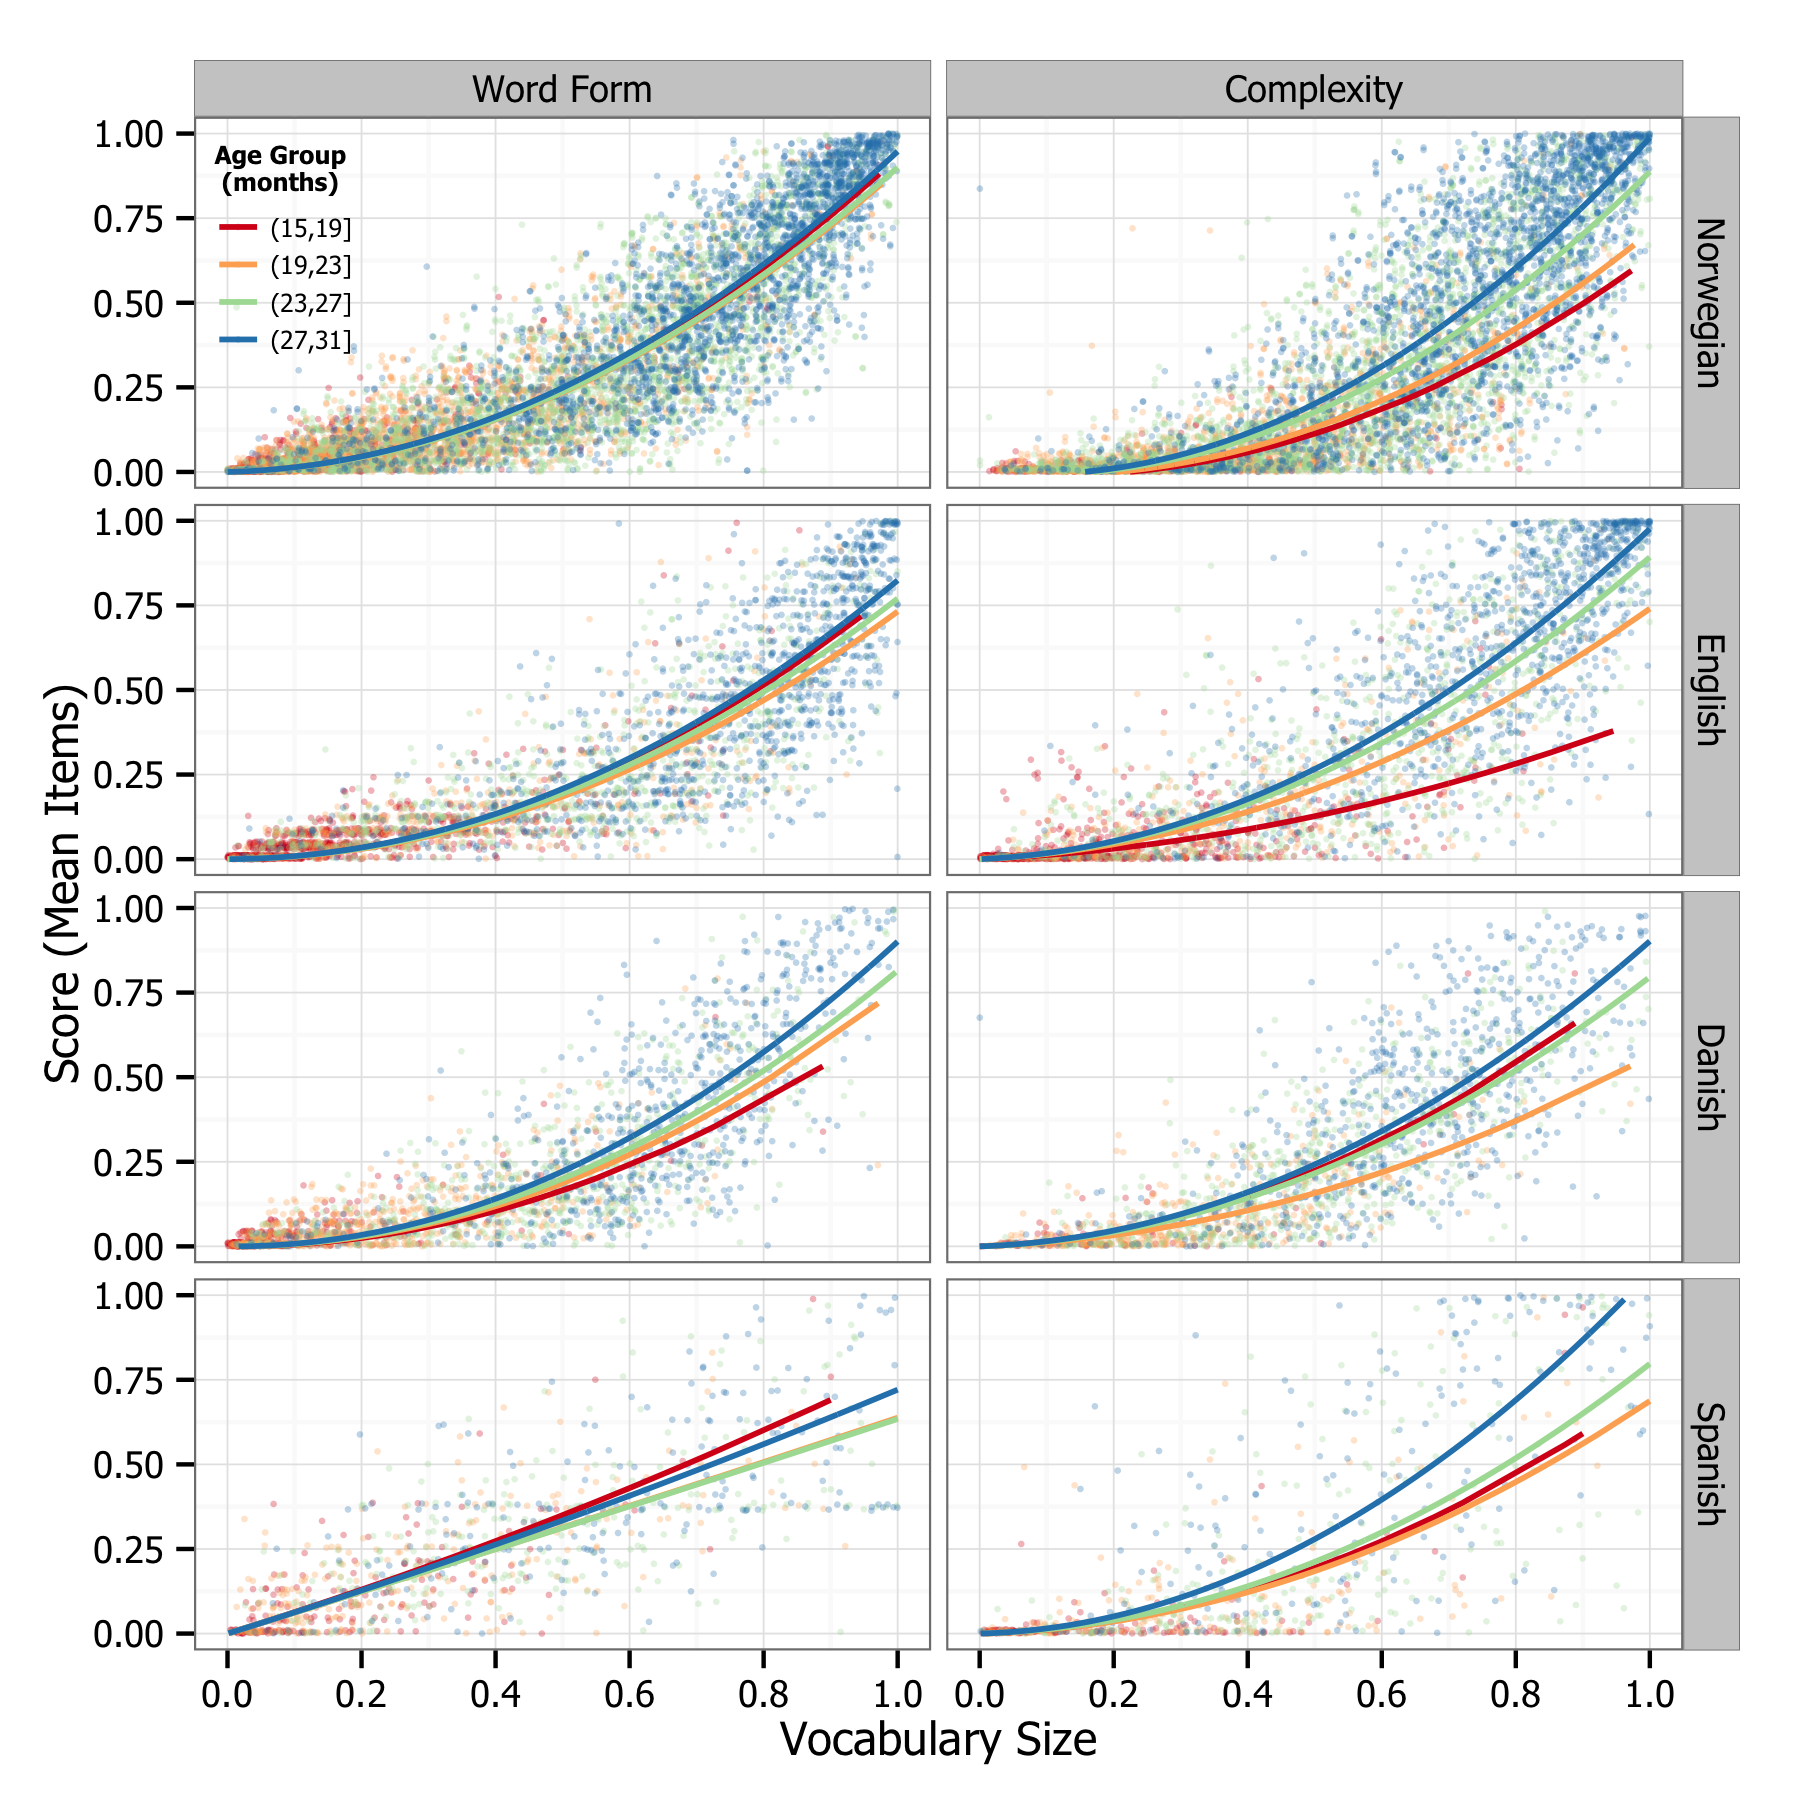
\includegraphics[width=.75\textwidth]{plots/grammar.png}
\caption{\label{fig:grammar} Each point shows an individual child, indicating their total vocabulary size and word form score or complexity score, with color showing their age bin (English $n=4137$; Spanish $n=1094$; Norwegian $n=8505$; Danish $n=2074$). Panels show different languages, and curves are regression models fit separately for each language and measure. The models were specified as \small{\tt{score $\sim$ vocab$^{2}$ * age}}.} 
\end{figure*}

By the age of two years, most children have a sizable working vocabulary, including verbs, prepositions and closed class forms that perform grammatical work functions. They are also beginning to use two- or three-word combinations (e.g., ``mommy sock'') and may demonstrate productive use of inflectional morphemes (e.g., past tense ``-ed''). As with vocabulary, there is sizable variation in when and how children move into grammar, and children who are more advanced in early vocabulary are more advanced in grammatical development as well \cite{bates1999}. This suggests that the mechanisms guiding vocabulary and grammar learning are highly interdependent \cite{tomasello2003,bresnan2001}, a view at odds with the nativist assumption that grammar emerges independent of the lexicon \cite{chomsky1981}.

Previous studies have found a strong connection between the size of the lexicon and grammatical development as measured by the complexity section of the CDI. A consistent non-linear relationship appears across a variety of languages, including English, Italian, Hebrew, and Spanish (see for a review). However, no studies have had the power and cross-linguistic representation to go beyond this initial finding. We extend it by examining grammatical development using two different measures: the word forms checklist as a window into morphology and the complexity checklist as a window into syntax. For each measure, we investigate the interaction of vocabulary size and age in a variety of languages.

\subsection{Results}

For each language in our sample, we wanted to estimate how much of a child's syntactic and morphological development was left to predicted after knowing that child's vocabulary size. Specifically, we asked whether knowing a child's age provided additional predictive power over and above vocabulary size. To estimate this predictive power of age, we fit regression models to each child's word-form and complexity scores. We modeled each child's score as a quadratic function of vocabulary size and interaction with the child's age in months. Figure~\ref{fig:grammar} shows a scatter plot of these data and models. Each dot represents an individual child's score on each measure, while curves show the relationship between that measure and vocabulary size. 

As seen most clearly for English and Norwegian, the curves for complexity show a characteristic fan, while the curves for word form show less of this fan, suggesting that the relationship between vocabulary size and complexity score is modulated by age, while the relationship between vocabulary size and word form score shows this pattern to a lesser extent. The Spanish and Danish data show less of a clear complexity curve fan, possibly because of the relatively small number of data points in the youngest age bin.

Because of the size of our samples, all main effects and interactions were highly significant in each language. To test our prediction---that vocabulary development predicts more of the variability in children's morphological than syntactic development---we compared the coefficients in our models across languages and measures. Figure~\ref{fig:coefs_grammar} shows the interaction between age and vocabulary size for each of these models across languages. In each model, the age-related interaction coefficient is substantially larger for complexity than for word form, indicating a greater developmental effect on complexity score. 

\begin{figure}[t]
\begin{center}
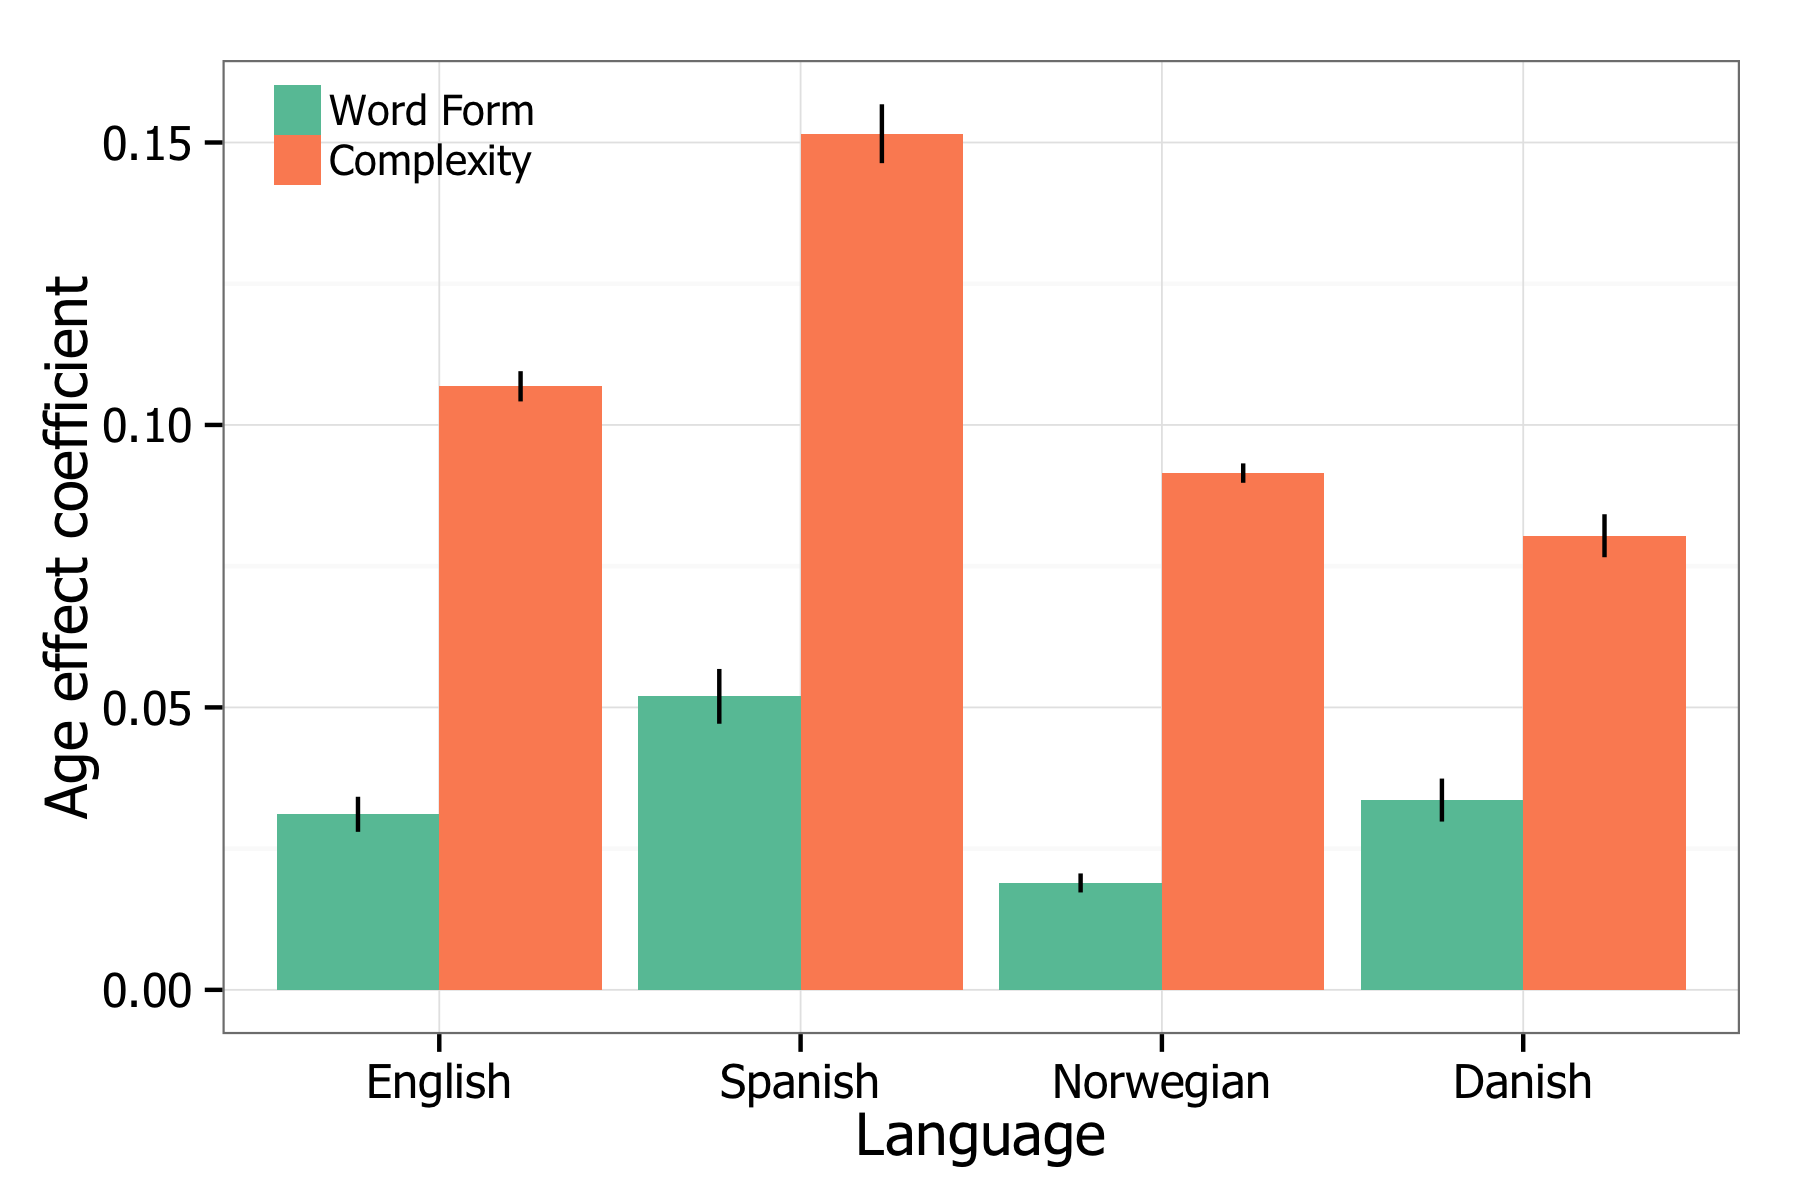
\includegraphics[width=\linewidth]{plots/coefs_wordform_complexity.png}
\end{center}
\caption{\label{fig:coefs_grammar}  For each language and measure (word form and complexity), the coefficient of the interaction between vocabulary size and age. Error bars show the standard error of the coefficient estimate. Across languages, complexity has a substantially larger interaction with age effect than word form, suggesting that less of children's syntactic development is predicted by their vocabulary growth.} 
\end{figure}

Given the heterogeneous nature of the CDI instruments, particularly of the complexity sections, we further break down the items of the complexity sections by classifying them as capturing more morphological or more syntactic phenomena. We then fit predictive models as above, but separately for each word form and complexity item. Figure \ref{fig:interactions} shows the z-score of the age-interaction terms of the models for each item. 

\begin{figure*}[t]
\centering
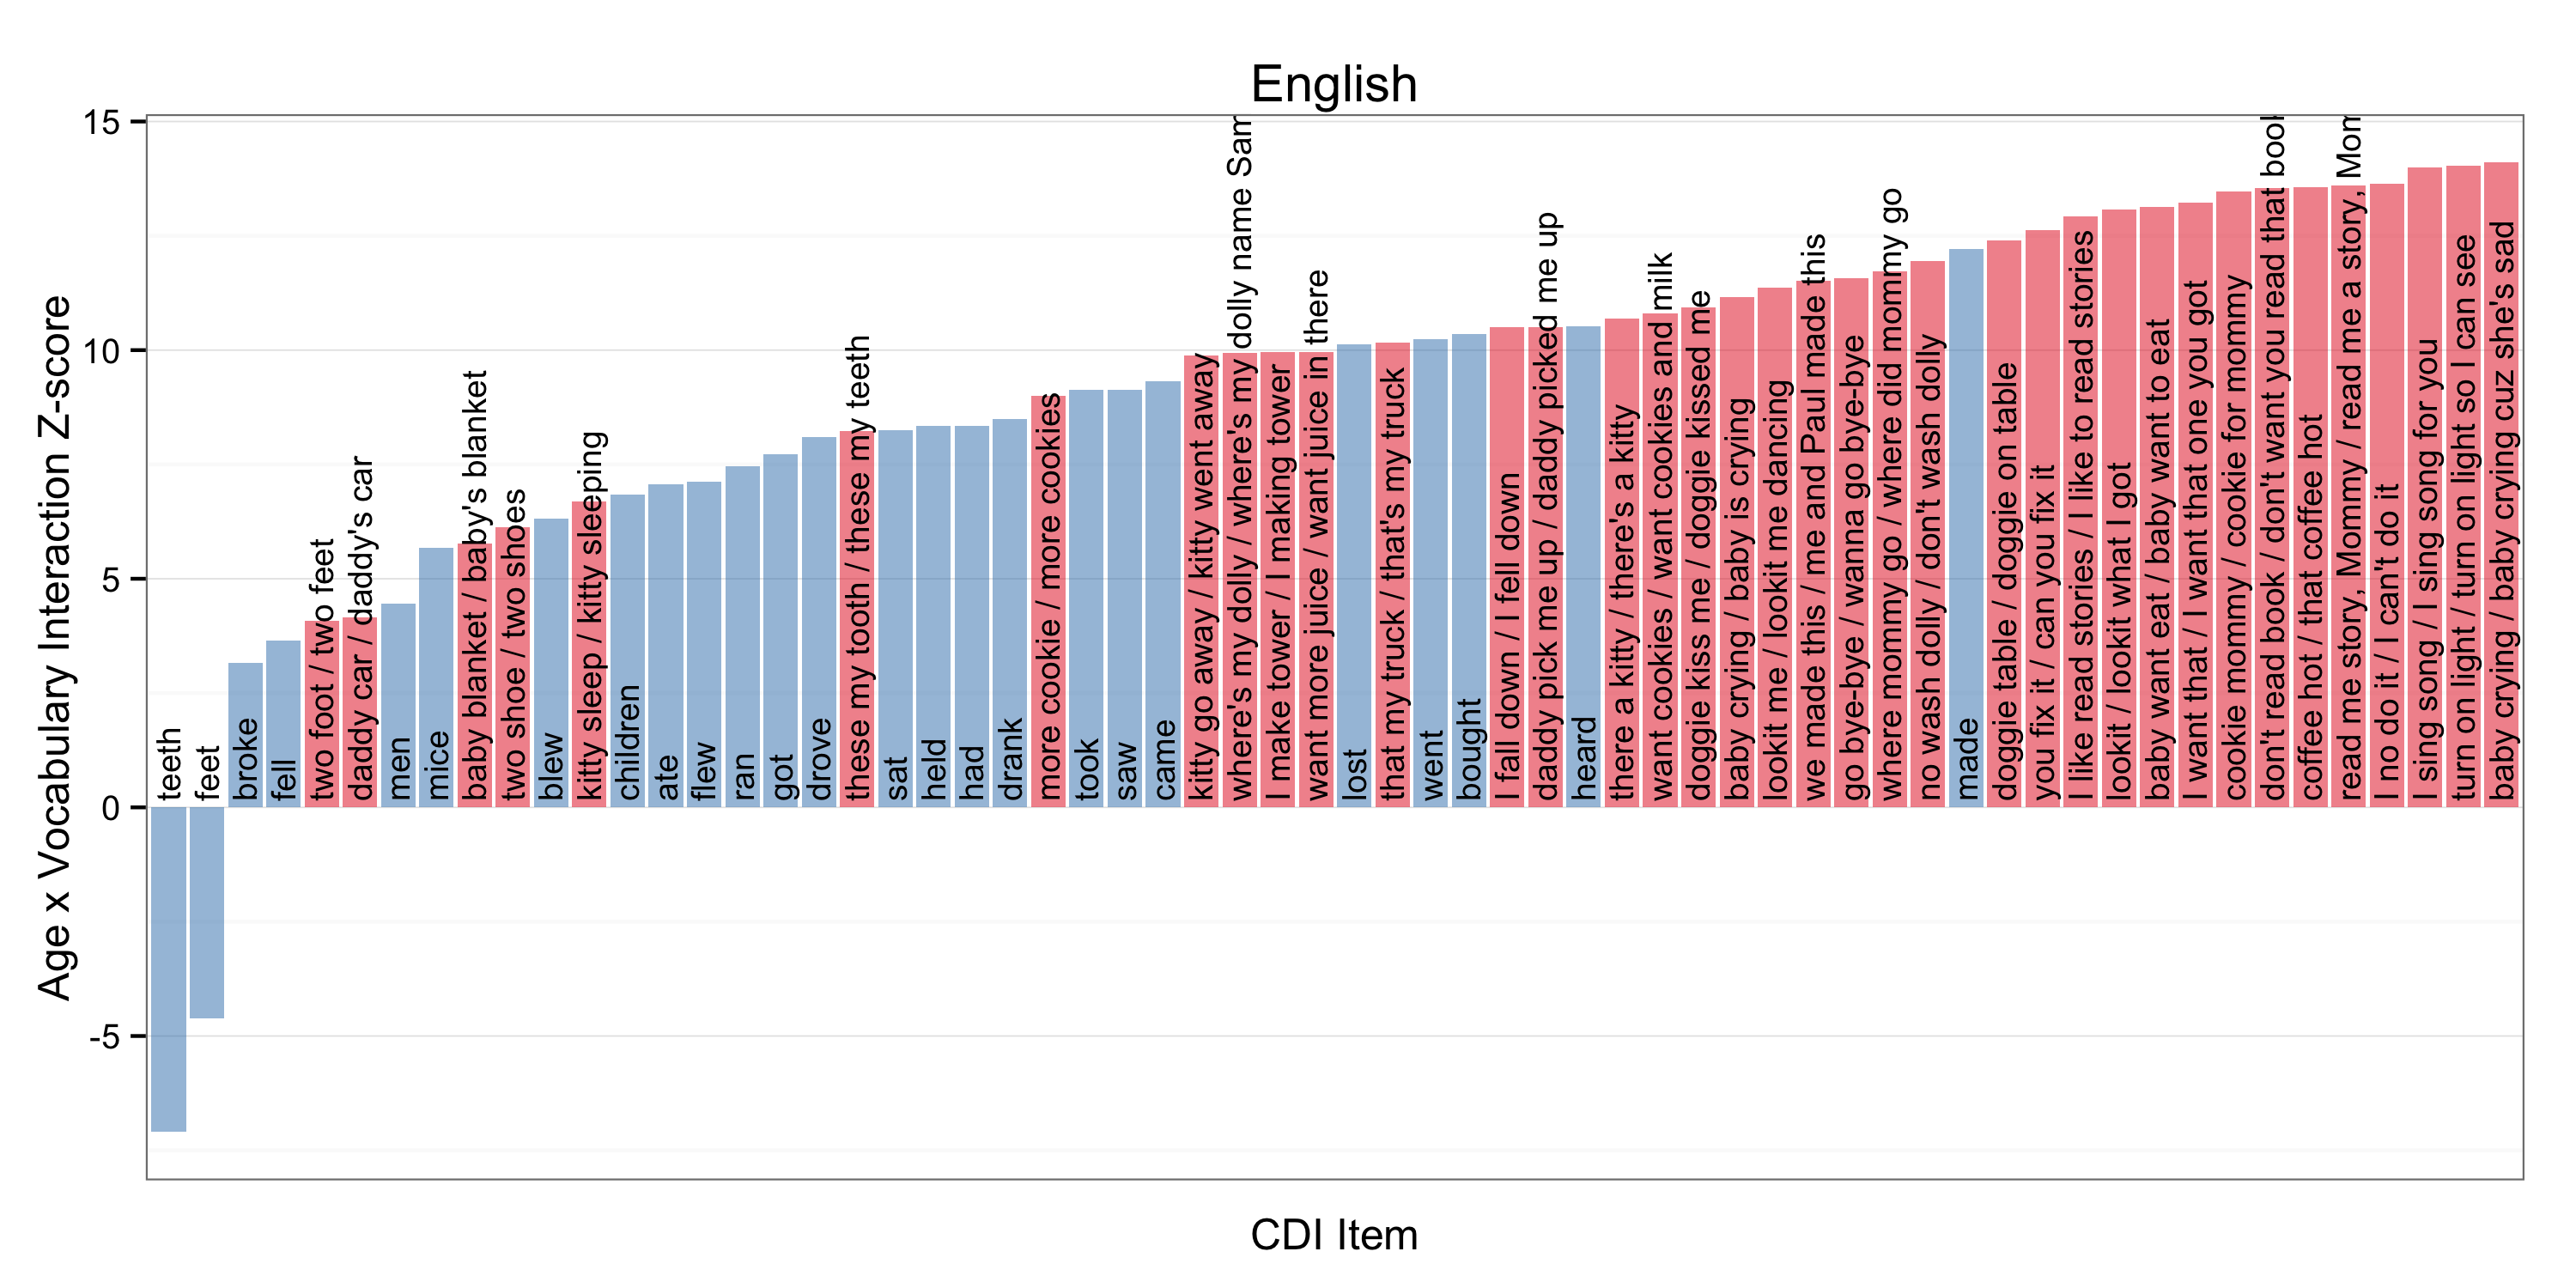
\includegraphics[width=.49\textwidth]{plots/english_interactions}
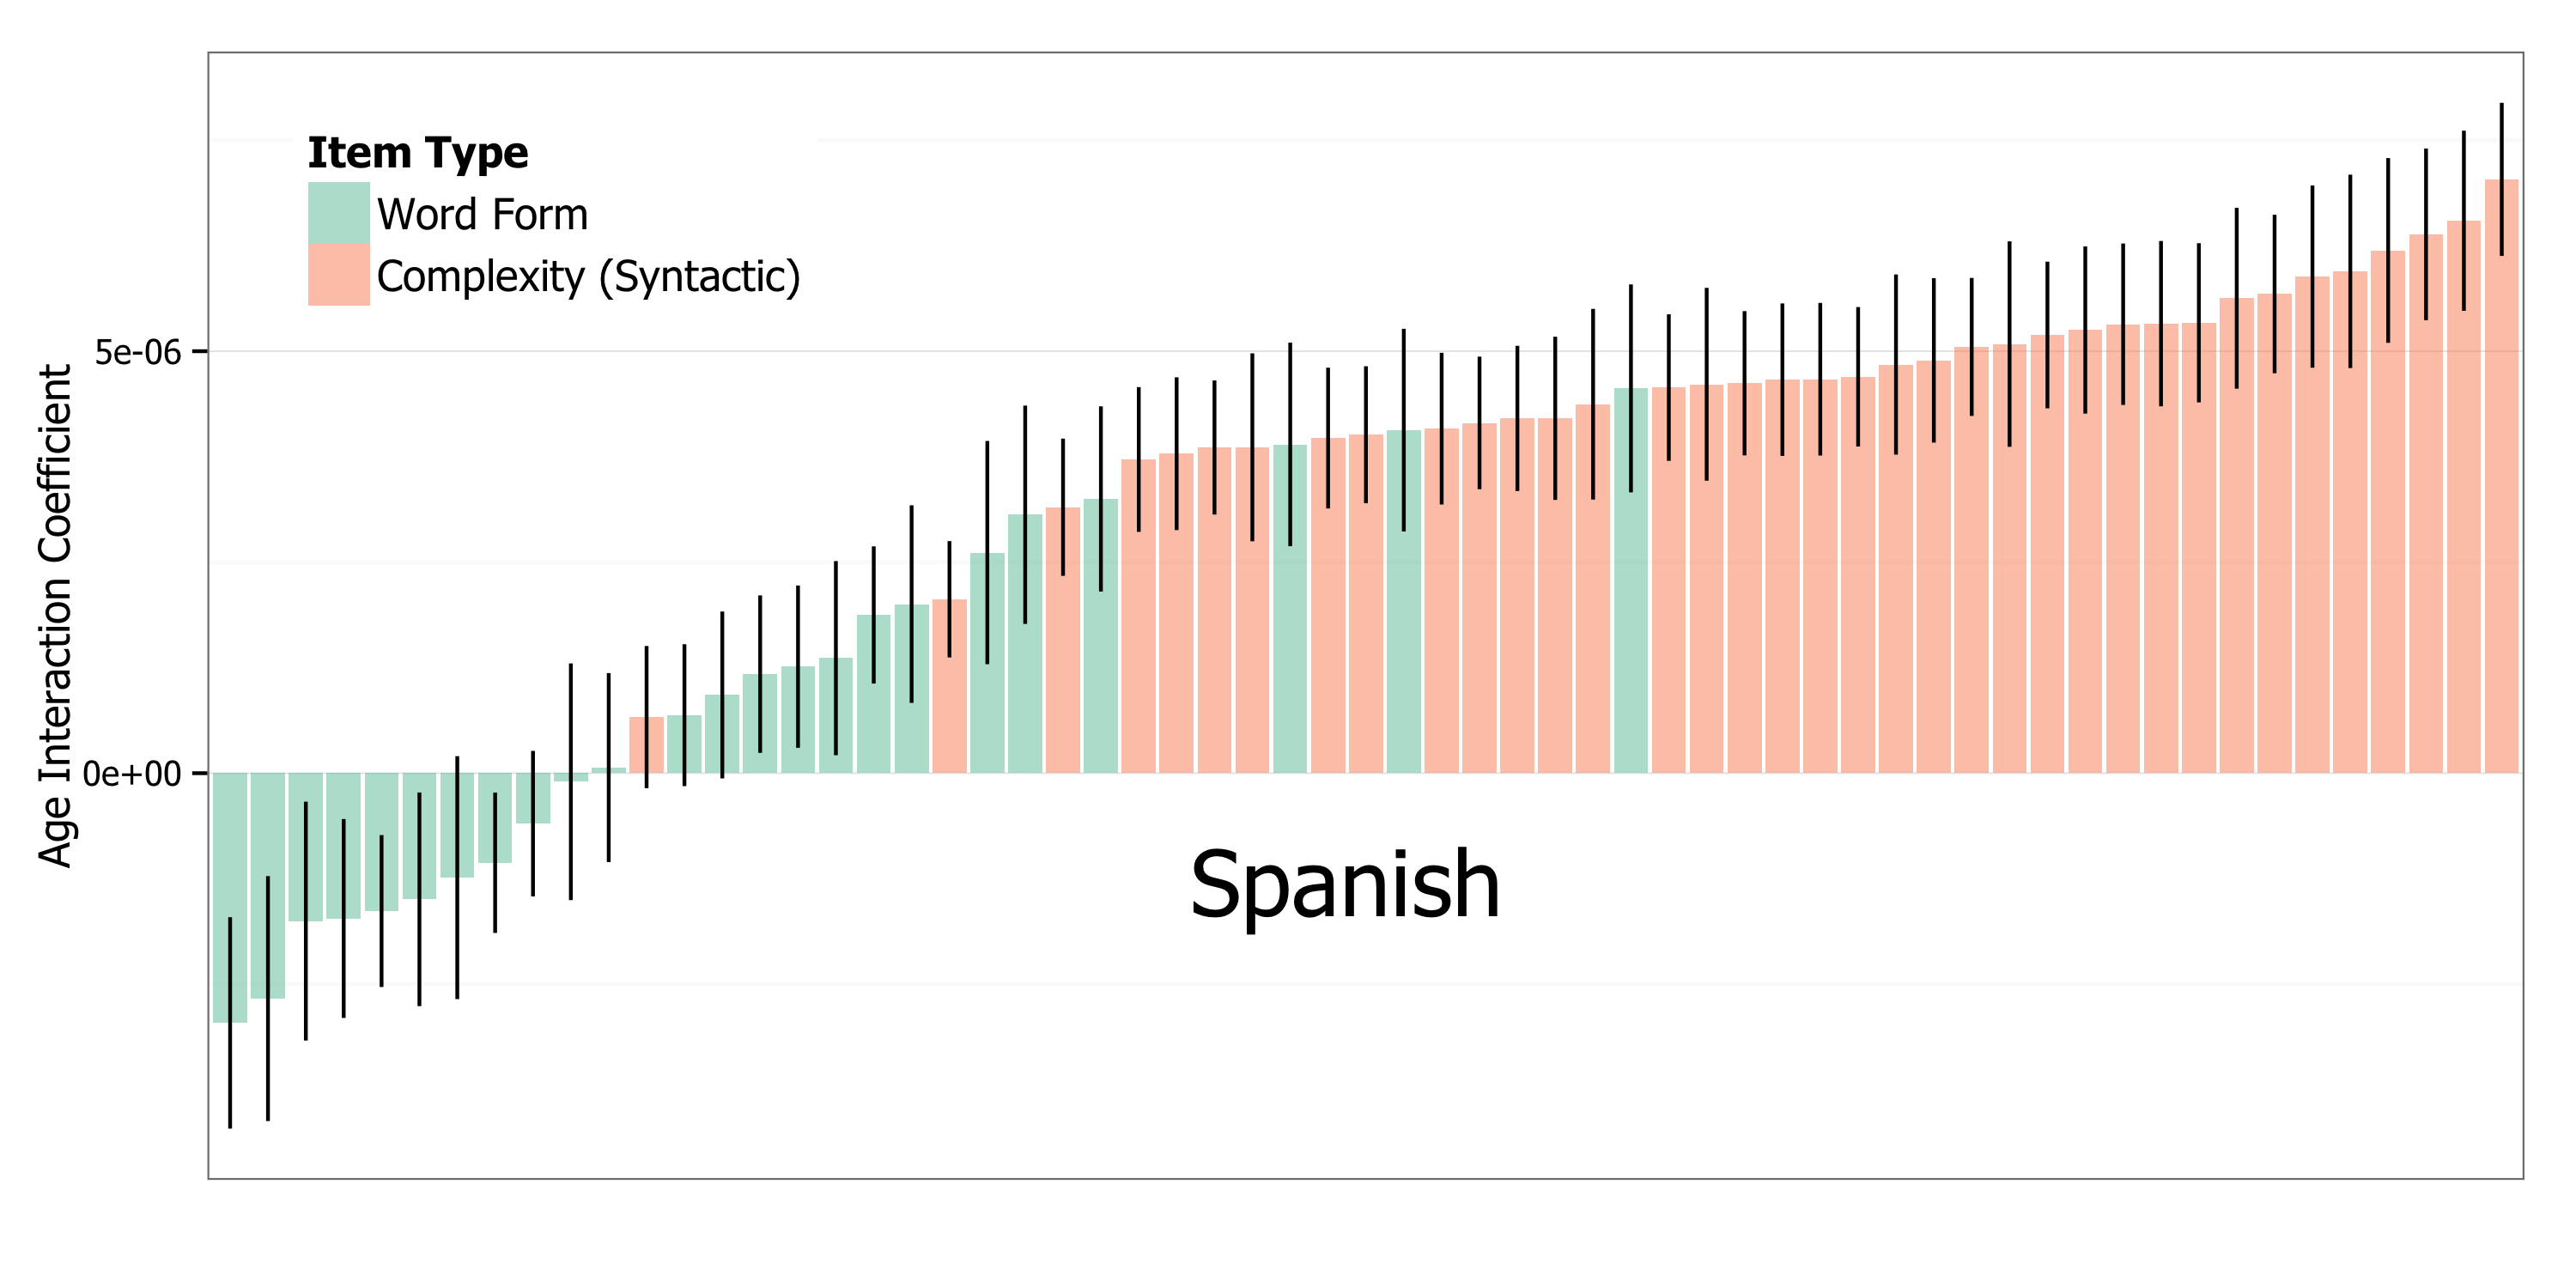
\includegraphics[width=.49\textwidth]{plots/spanish_interactions} \\
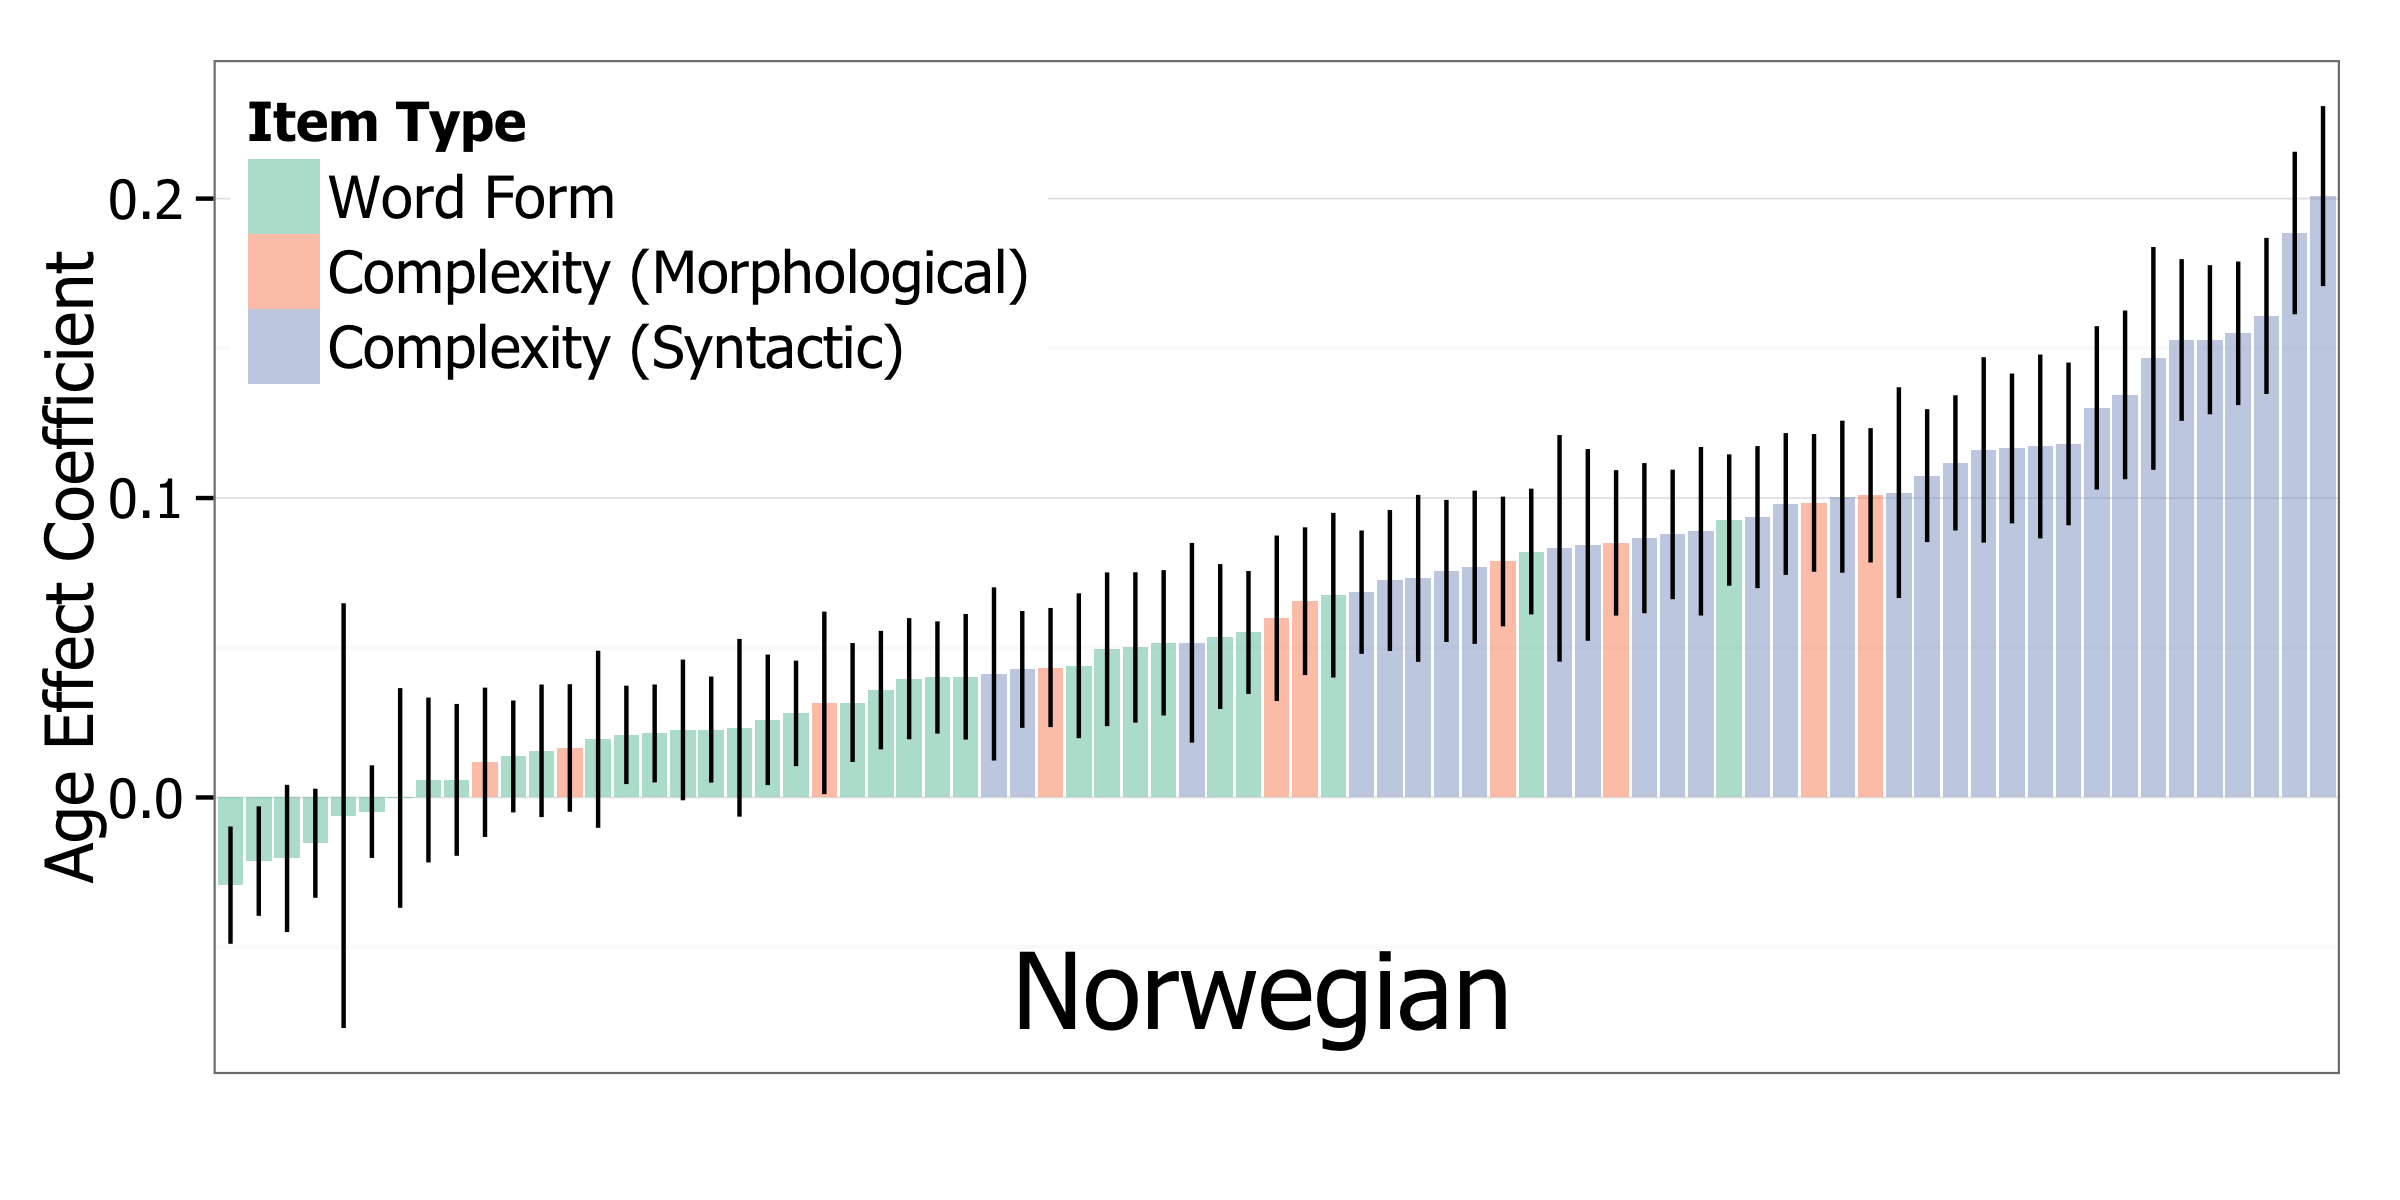
\includegraphics[width=.49\textwidth]{plots/norwegian_interactions}
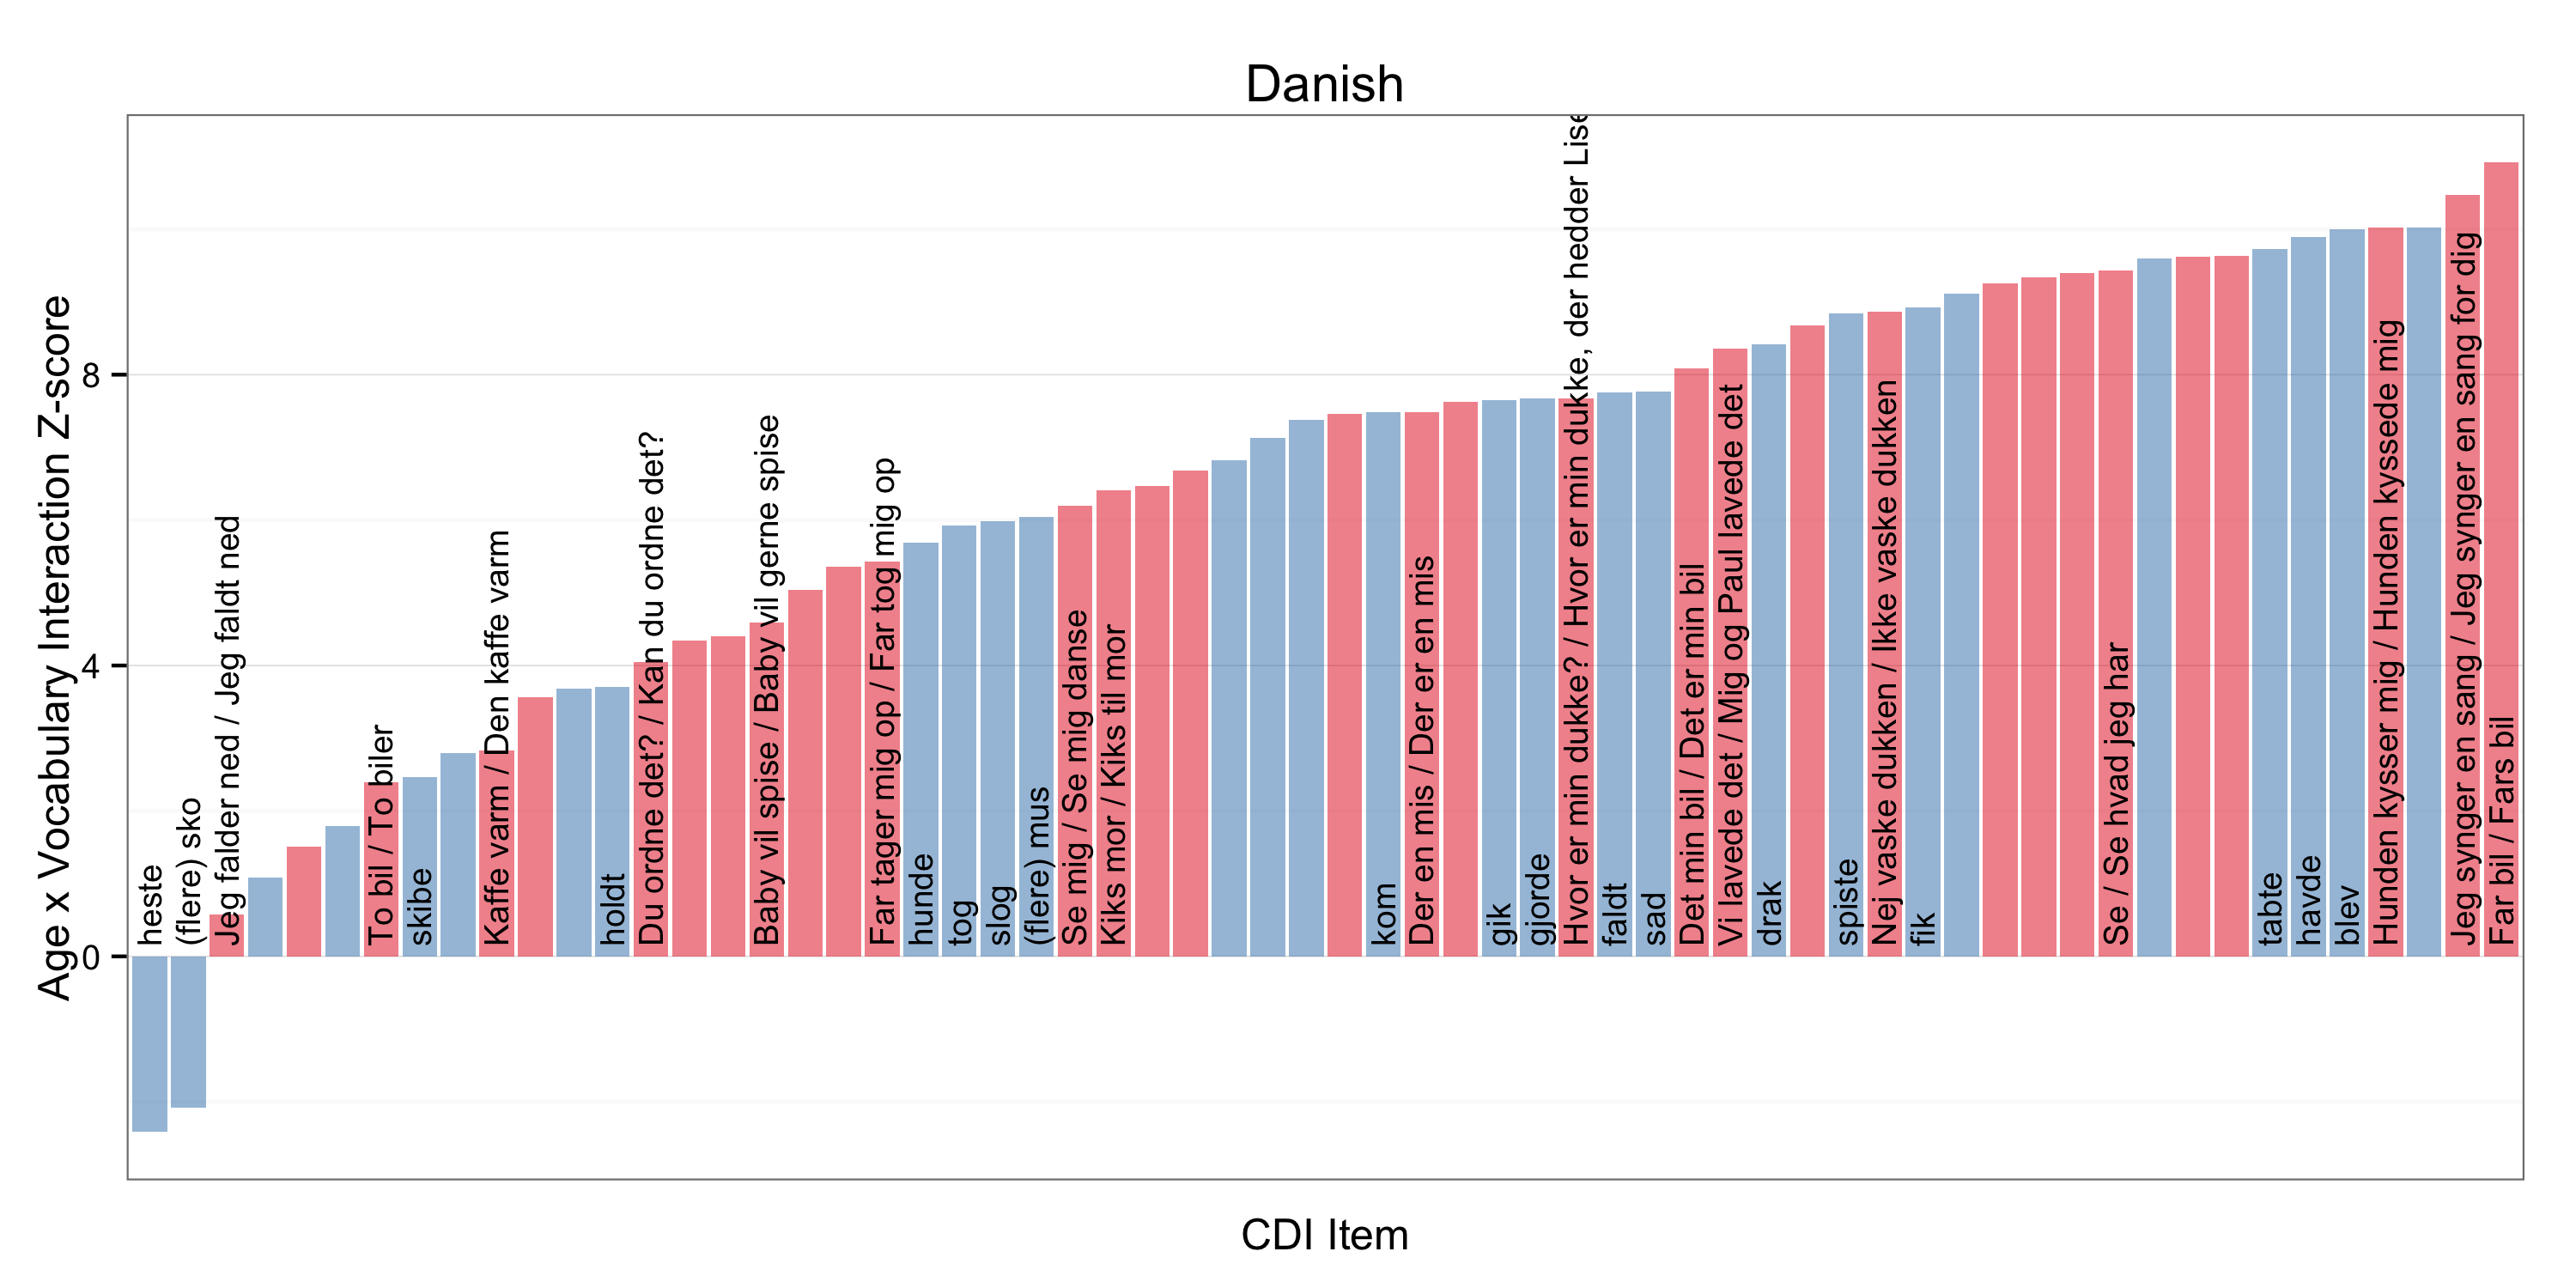
\includegraphics[width=.49\textwidth]{plots/danish_interactions}
\caption{\label{fig:interactions} For each language and item, the z-score of the model's age and vocabulary size interaction term. Across languages, complexity items tend to have a substantially larger age effect than word form items.}
\end{figure*}

\subsection{Discussion}

We build on previous analyses that showed a strong relationship between lexical and grammatical development, by factoring in the interplay of age with this relationship. We further distinguished in this analysis between measures more reflective of morphology and measures more reflective of syntax, and found that syntactic development broadly shows greater age modulation than morphological development. Thus, this analysis provides evidence for the relationship between syntactic development and age, independent of the growth of the lexicon. 

\section{Analysis 2: Vocabulary Composition}

\begin{figure*}[t]
\begin{center}
\includegraphics[width=\textwidth]{plots/composition.png}
\end{center}
\caption{\label{fig:vocab_comp} Proportion of a particular CDI category, plotted by total vocabulary size. Each point shows an individual child, with color showing their noun, predicate, and function word vocabulary. Panels show different languages, and curves are smoothing functions using loess (English $n=5595$; Spanish $n=1094$; Norwegian $n=10095$; Danish $n=3038$).} 
\end{figure*}

Early vocabulary development is typically characterized by learning of names for caregivers and common objects, while later in development, children tend to increase their vocabulary by increasing the proportion of predicates (verbs and adjectives). This over-representation of nouns has been found across a number of analyses and in a variety of languages \cite{bates1994}, though not all \cite{caselli1995}.\footnote{Differences in early vocabulary composition have been argued to emerge from typological differences (e.g., word order, subject drop), and from cultural practices (e.g., focus on picture book reading) \cite{tardif1999, gopnik1996, choi1995}---we are agnostic as to the source of this variability.}
For our purposes we are interested in using these analyses of vocabulary composition to test for the same kind of age-related differences that we found in the complexity and word-form analyses. 

We predict that the proportion of verbs in children's vocabulary should be relatively more affected by age than nouns. Concrete nouns are hypothesized to be learned initially from both co-occurrences between words \cite{yu2007b} and by social cues to reference to particular objects \cite{bloom2002}. On neither of these accounts should syntactic information be a primary information source (though of course syntax might be more informative for abstract nouns). In contrast, for verbs, syntax has been argued to be crucial for learning. On the syntactic bootstrapping hypothesis \cite{gleitman1990,fisher1994}, verbs are learned by  mapping the syntactic structure of utterances to the thematic structure of observed events, for example by noticing that the subject of a sentence matches the agent in one particular ongoing event but not another (``the cat is fleeing the dog'' matches  {\sc flees(cat, dog)} but not {\sc chases(dog,cat)}). Thus, if syntactic development is related in some way to age, we should see larger age effects on verb representation than noun representation. 

\subsection{Results}

Each CDI form contains a mixture of words in different classes. We adopt the categorization of \citeA{bates1994}, who split words in nouns, predicates (adjectives, adverbs, and verbs), function words, and other words. Then for each child's vocabulary, we compute the proportion of the total words in each of these categories that they are reported to produce. This yields a set of proportions for each child.

For each of the four languages in our sample, we plot these proportions against total vocabulary. These functions are shown in Figure \ref{fig:vocab_comp}: each dot represents an individual child's knowledge of a particular class, while curves show the relationship between that class and the entirety of the vocabulary. If categories grow independently of one another, these curves should approximate the diagonal. This pattern is not what either we or \citeauthor{bates1994} observe however: Across the languages in our sample, nouns are systematically over-represented in smaller vocabularies (shown by a curve that is above the diagonal), while function words---and to some extent, predicates---are under-represented. 

Next, we measure the contribution of age to vocabulary composition. We fit a linear model to all children's data for each word class, predicting word-class proportion as a linear and quadratic function of total vocabulary. We then investigated the interaction between total vocabulary and age. Because of our theoretical interest in the relationship between age and syntactic development, we focus here specifically on nouns and verbs. Figure \ref{fig:coefs_noun_verb} shows coefficients for each of these models across languages. In each model, the age-related interaction coefficient is substantially larger for verbs than for nouns. This asymmetry can be interpreted as evidence that for two vocabulary-matched children, the older would tend to have relatively more verbs than the younger, and this effect was larger for children with overall larger vocabularies. 

\subsection{Discussion}

We replicated previous analyses \cite{bates1994} showing an over-representation of nouns in the developing lexicon and a relative under-representation of verbs. We also predicted that---if syntactic generalization was in some way tied to age---verbs would show relatively more influence than nouns. This prediction was confirmed across all four languages we examined. Thus, this analysis provides additional circumstantial evidence for a relationship between syntactic development and age, independent of the growth of the lexicon.

\begin{figure}[!tb]
\centering
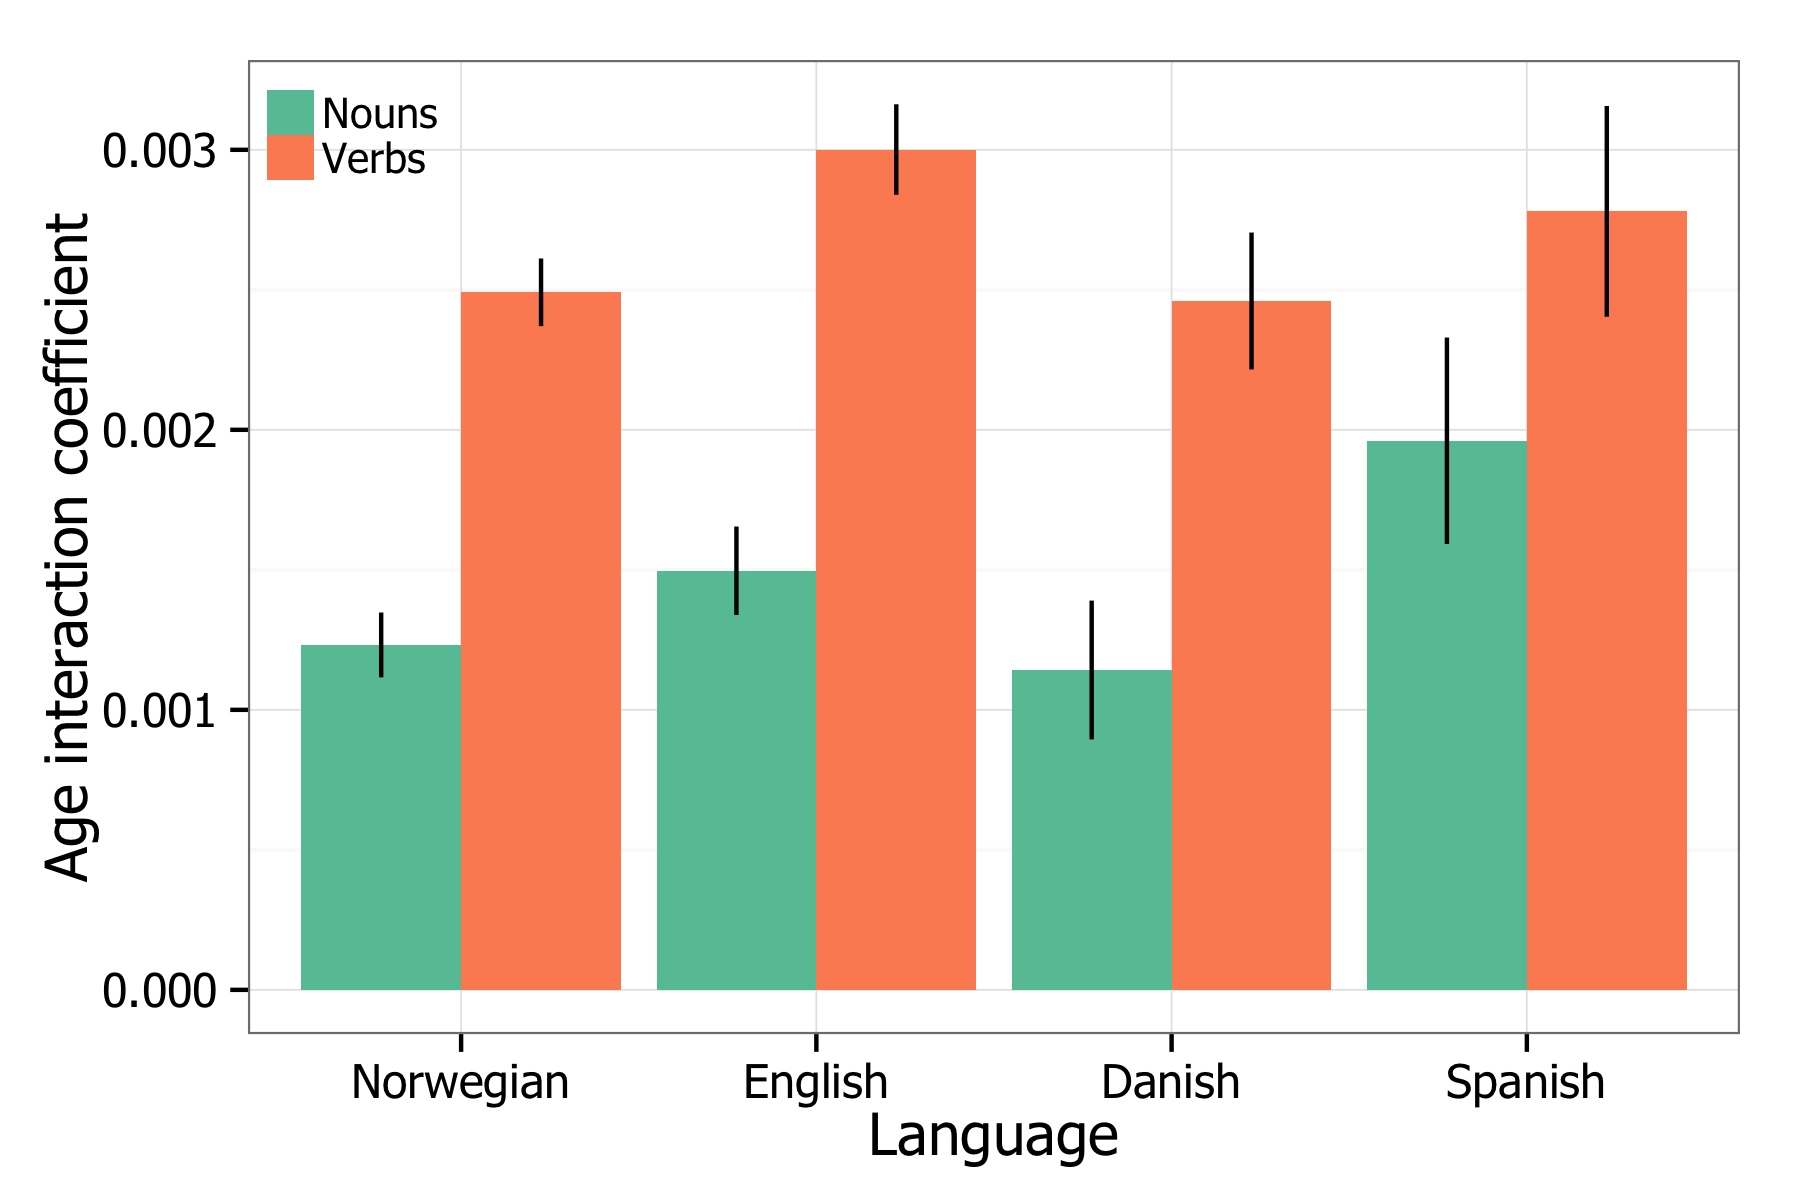
\includegraphics[width=\linewidth]{plots/coefs_noun_verb.png}
\caption{\label{fig:coefs_noun_verb} For each language and part of speech (nouns and verbs), the coefficient of the model's age and vocabulary size interaction term. Across languages, verbs have a substantially larger age effect than nouns. }
\end{figure}

\section{General Discussion}

We measured children's grammatical competence using different approaches: their reported usage of various morphological forms and syntactic constructions, and the substructure of their vocabularies by grammatical category. For each of these metrics, we used vocabulary size as a predictor and examined the interaction of age with this predictive relationship.

Across four languages, we find that syntax is modulated by age to a greater extent than morphology, and that verb proportion is modulated by age to a greater extent than noun proportion. Both of these findings suggest a place for developmental processes that facilitate grammatical acquisition, above vocabulary acquisition. This developmental change could range from something more domain-general like working memory to something more domain-specific like. In either case, it goes beyond a purely lexicalist account of grammatical acquisition.

\section{Acknowledgments}

Thanks to the MacArthur CDI Advisory Board, Dorthe Bleses, Kristian Kristoffersen, Rune N\o rgaard J\o rgensen, and the members of the Language and Cognition Lab. 

\bibliographystyle{apacite}

\setlength{\bibleftmargin}{.125in}
\setlength{\bibindent}{-\bibleftmargin}

\bibliography{CogSci}

\end{document}
